\chapter{Charts and Tables}
\section{Skill Roll Outcome Graph}
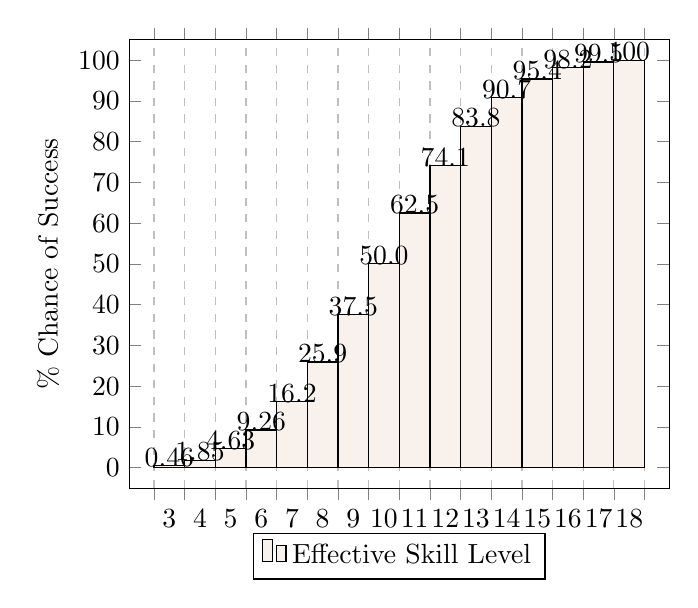
\begin{tikzpicture}
\begin{axis}[
	x tick label style={/pgf/number format/1000 sep=},
	ylabel=\% Chance of Success,
	enlargelimits=0.05,
	ytick = {0, 10, 20, 30, 40, 50, 60, 70, 80, 90, 100},
	legend style = {
	    at={(0.5,-0.1)},
	    grid style = dashed,
	    anchor=north,legend columns=-1
	},
	ybar interval = 1,
]
\addplot[fill = brown!10] 
	coordinates {
	    (3,    0.46) 
	    (4,    1.85)
		(5,    4.63) 
		(6,    9.26) 
		(7,   16.20) 
		(8,   25.93) 
		(9,   37.50) 
		(10,  50.00) 
		(11,  62.50) 
		(12,  74.07)
		(13,  83.80)
		(14,  90.74)
		(15,  95.37)
		(16,  98.15)
		(17,  99.54)
		(18, 100.00)
		(19, 0)
	};
\legend{Effective Skill Level}
\node at (3.5, 2.46) {0.46};
\node at (4.5, 3.85) {1.85};
\node at (5.5, 6.63) {4.63};
\node at (6.5, 11.26) {9.26};
\node at (7.5, 18.2) {16.2};
\node at (8.5, 27.9) {25.9};
\node at (9.5, 39.5) {37.5};
\node at (10.5, 52.0) {50.0};
\node at (11.5, 64.5) {62.5};
\node at (12.5, 76.1) {74.1};
\node at (13.5, 85.8) {83.8};
\node at (14.5, 92.74) {90.7};
\node at (15.5, 97.4) {95.4};
\node at (16.5, 100.2) {98.2};
\node at (17.5, 101.5) {99.5};
\node at (18.5, 102) {100};
\end{axis}
\end{tikzpicture}\\
The graph above shows the probability of succeeding a skill roll. If your character has an effective skill of 10, they have a 50\% chance of succeeding that roll. If they have a skill of 12, the chance of success goes up to 74\%.

\section{Critical Miss Table (Melee)}
\begin{center}
\begin{tabular}{r | l}
    \textbf{Roll} & \textbf{Result}\\\hline
    1 & Your weapon turns in your hand, and you hit with the flat side! \\
    2 & Your weapon breaks! \\
    3 & You lose your grip and the weapon flies out of your hand! \\
    4 & You lose your balance, and your turn! \\
    5 & You trip and fall! You have to get up again.\\
    6 & You hit yourself in the arm or leg! (50\% chance of hitting either)\\
\end{tabular}
\end{center}
\begin{note} 
    For \#3, the weapon flies 1d6 squares (50\% chance forward or backward). If it hits someone, it does half damage and lands there.
\end{note}

\section{Weapons} \label{sec:weapons}
\subsection{Melee Weapons}
\begin{center}
\begin{tabular}{c|c|c|c|c|c}
    \textbf{Category} & \textbf{Name} & \textbf{Class} & \textbf{Damage} & \textbf{Damage Type} & \textbf{Range} \\\hline
    Unarmed  & Fists          & Light & d6-2 & Crushing & Close/1\\
             & Feet           & Light & d6-1 & Crushing & Close/1\\\hline
    Medieval & Short Sword    & Light & d6   & Slashing & Close/1\\
             & Staff          & Light & d6-1 & Crushing & 1 to 2 \\
             & Long Sword     & Heavy & d6+2 & Slashing & 1 to 2 \\
             & Mace           & Heavy & d6+2 & Crushing & Close/1\\\hline
    Modern   & Baseball Bat   & Heavy & d6+1 & Crushing & Close/1\\
             & Aluminium Bat  & Light & d6+1 & Crushing & Close/1\\
             & Brass Knuckles & Light & d6-1 & Crushing & Close/1\\\hline
    Future   & Beam Sword     & Light & d6+3 & Slashing & Close/1
\end{tabular}
\end{center}

\subsection{Ranged Weapons}
\begin{center}
\begin{tabular}{c|c|c|c|l}
    \textbf{Category} & \textbf{Name} & \textbf{Damage} & \textbf{Damage Type} & \textbf{Accurate Range} \\\hline
    Primitive & Rock        & d6-1  & Crushing & $0.5 \times Shooting + Prof$  \\\hline
    Medieval  & Short Bow   & d6+1  & Piercing & $Shooting + Prof$ \\
              & Long Bow    & d6+2  & Piercing & $2 \times Shooting + Prof$ \\\hline
    Modern    & Pistol      & 2d6+2 & Ballistic & 56m \\
              & Shotgun     & 5d6   & Ballistic & 3m \\\hline
    Future    & Laser Gun   & 6d6   & Piercing & 66m \\
\end{tabular}
\end{center}
\begin{note} 
    These ranges are for when you want to shoot without a range penalty.
    So despite the fact that a pistol can shoot around 1800m, it's incredibly hard to do so.
\end{note}

\section{Armour} \label{sec:armour}
\begin{center}
\begin{tabular}{c|c|c|l}
\textbf{Category} & \textbf{Name}  & \textbf{DfM} & \textbf{DR}\\\hline
         Medieval & Leather        & 1 & 1 to Cr.\\
                  & Studded Leather& 1 & 2 to Cr.\\
                  & Half Plate     & 2 & 2 ex. Ba.\\
                  & Full Plate     & 4 & 3 \\
                  & Chain Mail     & 1 & 1 ex. Pi. \& Ba.\\\hline
           Modern & Summer Clothes & 0 & 0 \\
                  & Winter Clothes & 0 & 1 ex. Ba.\\
                  & Kevlar Vest    & 1 & 3 to Ba.\\\hline
           Future & Polymer        & 4 & 3 \\
\end{tabular}
\end{center}

\section{Shields} \label{sec:shields}
\begin{center}
    \begin{tabular}{c|c|c|c|c|c|l}
        \textbf{Category} & \textbf{Name} & \textbf{Class} & \textbf{Damage} & \textbf{Damage Type} & \textbf{DfM} & \textbf{DR} \\\hline
        Medieval & Buckler          & Light & d6-2 & Crushing & 1 & 1 ex. Ba.\\
                 & Wooden Shield    & Light & d6-1 & Crushing & 2 & 1 ex. Ba.\\
                 & Spiked Shield    & Heavy & d6+1 & Piercing & 2 & 2 ex. Ba.\\
                 & Tower Shield     & Heavy & d6   & Crushing & 4 & 4\\\hline
        Modern   & Riot Shield      & Light & d6/2 & Crushing & 2 & 1 ex. Ba.\\
                 & Ballistic Shield & Heavy & d6   & Crushing & 3 & 5\\
                 & Car Door         & Heavy & d6+3 & Crushing & 3 & 3 ex. Ba.\\\hline
        Future   & Energy Shield    & Light & 2d6  & Crushing & 5 & 5 ex. Pi \& Sl.
    \end{tabular}
\end{center}

\section{Combat Order Reference}\label{sec:combat-order}
\begin{center}
\begin{tabular}{l}
    \multicolumn{1}{c}{\textbf{Initiative}}\\
    Each player rolls $1d6 + Athletics \pm Modifiers$ to determine turn order.\\
    Whoever is first in the turn order, enters the \textit{Proactive Phase}.\\\hline\\
    \multicolumn{1}{c}{\textbf{Proactive Phase}}\\
    Select two of the following: Move, Brace, Attack.\\
    If the action solicits a response, go to the \textit{Reactive Phase}.\\
    If the action solicits no response, go to the next player's \textit{Proactive Phase}.\\\hline\\
    \multicolumn{1}{c}{\textbf{Reactive Phase}}\\
    Select up to two of the following: Dodge, Parry, Counter.\\
    If damage is avoided, the next player's \textit{Proactive Phase} starts.\\
    If damage is \textit{not} avoided, go to \textit{Damage Calculations}.\\\hline\\
    \multicolumn{1}{c}{\textbf{Damage Calculations}}\\
    Attacker rolls the relevant damage dice.\\
    Defender subtracts damage resistance from attacker's result.\\
    Defender subtracts that many hit-points from their health.\\
    Next player's \textit{Proactive Phase} starts.\\
\end{tabular}
\end{center}